\documentclass[border=5mm,tikz]{standalone}
\usepackage{tikz-cd}
\usepackage{amsmath}

\begin{document}

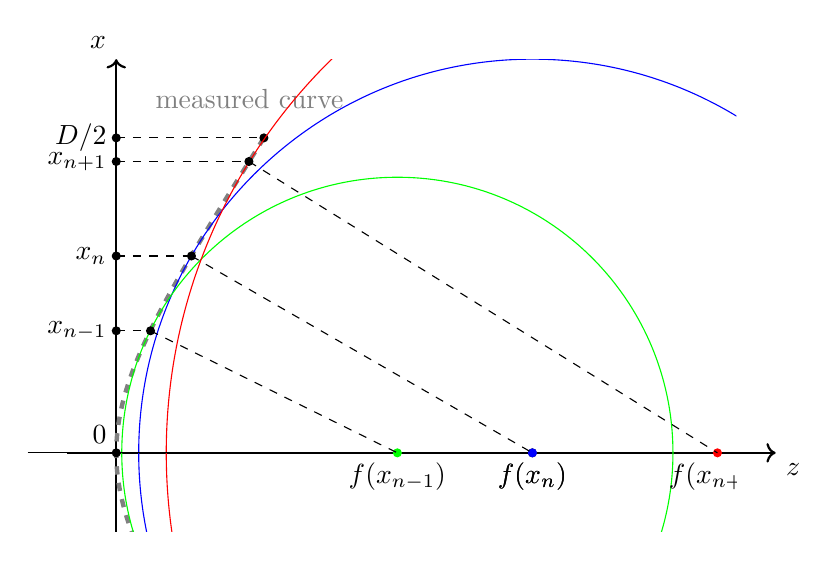
\begin{tikzpicture}

\draw[thick,->] (-1,0) -- (8,0) node[anchor=north west] {$z$};
\draw[thick,->] (-0.375,-1) -- (-0.375,5) node[anchor=south east] {$x$};

\begin{scope}
\clip (-1.5,-1) rectangle (7.5,5);

\draw[ultra thick, gray, dashed] (1.5, 4) .. controls (-1, 0) .. (1.5, -4);

\node [right, gray] at (0, 4.5) {measured curve};

\draw[fill] (4.91,0) circle [radius=0.05];
\node [below] at (4.91,0) {$f(x_n)$};

\draw[fill] (-0.375,0) circle [radius=0.05];
\node [above left] at (-0.375,0) {$0$};

\draw[fill] (-0.375,4) circle [radius=0.05];
\node [left] at (-0.375,4) {$D/2$};
\draw[fill] (1.5,4) circle [radius=0.05];
\draw[dashed] (-0.375,4) -- (1.5,4);

%Measurement 1
\draw[blue] (4.91,0) circle (5);

\draw[blue, fill] (4.91,0) circle [radius=0.05];
\node [below] at (4.91,0) {$f(x_n)$};

\draw[fill] (0.58,2.5) circle [radius=0.05];

\draw[fill] (-0.375, 2.5) circle [radius=0.05];
\node [left] at (-0.375, 2.5) {$x_n$};

\draw[dashed] (-0.375,2.5) -- (0.58,2.5);

\draw[dashed] (0.58,2.5) -- (4.91,0);

%Measurement 2
\draw[green] (3.195,0) circle (3.5);

\draw[green, fill] (3.195,0) circle [radius=0.05];
\node [below] at (3.195,0) {$f(x_{n-1})$};

\draw[fill] (0.06,1.55) circle [radius=0.05];

\draw[fill] (-0.375, 1.55) circle [radius=0.05];
\node [left] at (-0.375, 1.55) {$x_{n-1}$};

\draw[dashed] (-0.375,1.55) -- (0.06,1.55);

\draw[dashed] (0.06,1.55) -- (3.195,0);

%Measurement 3
\draw [red] (7.26,0) circle (7);

\draw[red, fill] (7.26,0) circle [radius=0.05];
\node [below] at (7.26,0) {$f(x_{n+1})$};

\draw[fill] (1.31,3.7) circle [radius=0.05];

\draw[fill] (-0.375, 3.7) circle [radius=0.05];
\node [left] at (-0.375, 3.7) {$x_{n+1}$};

\draw[dashed] (-0.375,3.7) -- (1.31,3.7);

\draw[dashed] (1.31,3.7) -- (7.26,0);

\draw (-1.5,0) -- (1.5,0);

\end{scope}

\end{tikzpicture}

\end{document}